\documentclass[journal]{IEEEtran}
\usepackage[english]{babel}

\usepackage{amssymb, amsmath} %Paquetes matemáticos de la American Mathematical 
\usepackage[utf8]{inputenc}
\usepackage{graphicx}
\usepackage{float}
\usepackage{hyperref}
\usepackage{listings}
\usepackage{xcolor}

\definecolor{codegreen}{rgb}{0,0.6,0}
\definecolor{codegray}{rgb}{0.5,0.5,0.5}
\definecolor{codepurple}{rgb}{0.58,0,0.82}
\definecolor{backcolour}{rgb}{0.95,0.95,0.92}
% Definicio de estilo para el codigo fuente que se cita
\lstdefinestyle{mystyle}{
    backgroundcolor=\color{backcolour},   
    commentstyle=\color{codegreen},
    keywordstyle=\color{magenta},
    numberstyle=\tiny\color{codegray},
    stringstyle=\color{codepurple},
    basicstyle=\ttfamily\footnotesize,
    breakatwhitespace=false,         
    breaklines=true,                 
    captionpos=b,                    
    keepspaces=true,
    numbers=left,                    
    numbersep=5pt,                  
    showspaces=false,                
    showstringspaces=false,
    showtabs=false,                  
    tabsize=2,
}
\lstset{style=mystyle}

\renewcommand{\lstlistingname}{Código}

\ifCLASSINFOpdf

\else

\fi
\begin{document}

\title{Ejercicio 2 - tema 6 \\ Estructuras lógicas de almacenamiento - Segmentos}
%
\author{Vicente Romero Andrade}

\markboth{Ejercicio 2 - tema 6 Estructuras lógicas de almacenamiento - Segmentos, Julio~2021}%
{Shell \MakeLowercase{\textit{et al.}}: }
% The only time the second header will appear is for the odd numbered pages

\maketitle


\IEEEpeerreviewmaketitle

\section{Objetivo}
% The very first letter is a 2 line initial drop letter followed

\IEEEPARstart{E}{l} objetivo es comprender el mecanismo de creación de los distintos 
tipos de segmentos a partir de la creación de una tabla. Explorar las vistas del diccionario
de datos para verificar la creación de segmentos asociados a los objetos de un usuario.

\section{Desarrollo}
\subsection{sentencias}
\begin{lstlisting}[language=sql, caption=s-00-crea-usuario.sql,label={lst:codigo1}]
connect sys/system2 as sysdba
CREATE USER VRA0602 IDENTIFIED BY VRA0602 quota unlimited on users;
GRANT CONNECT TO VRA0602;
GRANT CREATE TABLE TO VRA0602;
\end{lstlisting}
\begin{lstlisting}[language=sql, caption=s-01-crear-tabla.sql,label={lst:codigo2}]
whenever sqlerror exit rollback
set serveroutput on
connect VRA0602/VRA0602
-- B
declare
  v_count number;
  v_username varchar2(30) := 'VRA0602';
  v_table varchar2(30) := 'EMPLEADO';
begin
  --Verificar si la table existe
  select count(*) into v_count
  from all_tables
  where table_name = v_table
  and owner = v_username;
  --Si existe la tabla, entonces se borra
  if v_count > 0 then
    execute immediate 'drop table '||v_table;
  end if;
  execute immediate 'create table '||v_table||' (
    id number,
    nombre_completo varchar2(80) not null,
    num_cuenta varchar2(9),
    expediente clob,
    constraint pk_empleado primary key(id),
    constraint empleado_num_cuenta_uk unique(num_cuenta)
  )';
end;
/
insert into empleado(id,nombre_completo,num_cuenta,expediente) values (1,'Vicente Romero Andrade','312097792',null);
commit;
-- C
select 
        SEGMENT_NAME, 
        SEGMENT_TYPE, 
        TABLESPACE_NAME,
        BYTES,
        BLOCKS,
        EXTENTS 
    from USER_SEGMENTS 
        where SEGMENT_NAME like '%EMPLEADO%';
-- D
select
        SEGMENT_NAME,
        SEGMENT_TYPE,
        TABLESPACE_NAME,
        BYTES,
        BLOCKS,
        EXTENTS
    from USER_SEGMENTS
        where SEGMENT_NAME like '%EMPLEADO%'
          or SEGMENT_NAME in (select SEGMENT_NAME from USER_LOBS ul where ul.TABLE_NAME = 'EMPLEADO')
          or SEGMENT_NAME in (select INDEX_NAME from USER_LOBS ul where ul.TABLE_NAME = 'EMPLEADO');
whenever sqlerror continue
\end{lstlisting}
\begin{figure}[H]
  \centering
  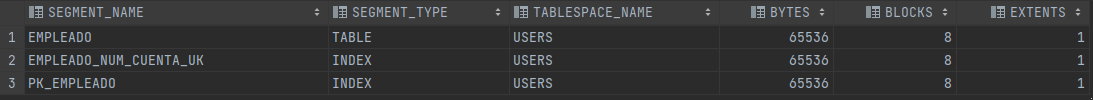
\includegraphics[scale=.22]{captura_1.png}
   \caption{respuesta inciso C}
   \label{fig:validador_1}
\end{figure}

\subsection{C2. s-02-conexiones.sql y tnsnames.ora}

\begin{lstlisting}[language=sql, caption=s-02-conexiones.sql,label={lst:codigo3}]
  whenever sqlerror exit rollback
  set serveroutput on
  connect sys@vrabda2_dedicated/system2 as sysdba
  
  declare
    v_count number;
    v_username varchar2(30) := 'VRA0501';
    v_table varchar2(30) := 'T01_SESSION_DATA';
  begin
    --Verificar si la table existe
    select count(*) into v_count
    from all_tables
    where table_name = v_table
    and owner = v_username;
    --Si existe la tabla, entonces se borra
    if v_count > 0 then
      execute immediate 'drop table '|| v_username ||'.'||v_table;
    end if;
    execute immediate 'create table '|| v_username ||'.'||v_table||'(
      id number,
      sid number,
      logon_time date,
      username varchar2(20),
      status varchar2(8),
      server varchar2(20),
      osuser varchar2(30),
      process varchar2(12),
      port number
  )';
  end;
  /
  -- A
  insert into vra0501.t01_session_data(
  id,sid,logon_time,username,status,server,
  osuser,process,port)
  select 1,sid,logon_time,username,status,server,
      osuser,process,port from v$session where username = 'SYS';
  commit;
  --B
  connect sys@vrabda2_shared/system2 as sysdba
  
  insert into vra0501.t01_session_data(
  id,sid,logon_time,username,status,server,
  osuser, process,port) 
  select 2,sid,logon_time,username,status,server,
      osuser, process,port from v$session where username = 'SYS';
  commit;
  
  --C
  connect VRA0501@vrabda2_dedicated/VRA0501
  
  insert into vra0501.t01_session_data(
  id,sid,logon_time,username,status,server,
  osuser, process,port) 
  select 3,sid,logon_time,username,status,server,
      osuser, process,port from v$session where username = 'VRA0501';
  commit;
  
  --D
  connect VRA0501@vrabda2_shared/VRA0501
  
  insert into vra0501.t01_session_data(
  id,sid,logon_time,username,status,server,
  osuser, process,port) 
  select 4,sid,logon_time,username,status,server,
      osuser, process,port from v$session where username = 'VRA0501';
  commit;
  
  whenever sqlerror continue  
\end{lstlisting}
\begin{lstlisting}[language=bash, caption=tnsname.ora,label={lst:codigo2}]
  # tnsnames.ora Network Configuration File: /u01/app/oracle/product/19.0.0/dbhome_1/network/admin/tnsnames.ora
  # Generated by Oracle configuration tools.
  
  VRABDA1 =
    (DESCRIPTION =
      (ADDRESS = (PROTOCOL = TCP)(HOST = pc-vra.fi.unam)(PORT = 1521))
      (CONNECT_DATA =
        (SERVER = DEDICATED)
        (SERVICE_NAME = vrabda1.fi.unam)
      )
    )
  
  LISTENER_VRABDA1 =
    (ADDRESS = (PROTOCOL = TCP)(HOST = pc-vra.fi.unam)(PORT = 1521))
  
  VRABDA2 =
    (DESCRIPTION =
      (ADDRESS = (PROTOCOL = TCP)(HOST = pc-vra.fi.unam)(PORT = 1521))
      (CONNECT_DATA =
        (SERVER = DEDICATED)
        (SERVICE_NAME = vrabda2)
      )
    )
  
  VRABDA2_DEDICATED =
          (DESCRIPTION =
                  (ADDRESS_LIST =
                          (ADDRESS = (PROTOCOL = TCP)(HOST = pc-vra.fi.unam)(PORT = 1521))
                  )
          (CONNECT_DATA =
                  (SERVICE_NAME = vrabda2)
                  (SERVER=DEDICATED)
          )
  )
  
  VRABDA2_SHARED =
          (DESCRIPTION =
                  (ADDRESS_LIST =
                          (ADDRESS = (PROTOCOL = TCP)(HOST = pc-vra.fi.unam)(PORT = 1521))
                  )
          (CONNECT_DATA =
                  (SERVICE_NAME = vrabda2)
                  (SERVER=SHARED)
          )
  )
\end{lstlisting}
\subsection{C3. s-03-consultas.sql}
\begin{lstlisting}[language=sql, caption=s-03-consultas.sql,label={lst:codigo5}]
whenever sqlerror exit rollback
set serveroutput on
connect sys/system2 as sysdba

declare
  v_count number;
  v_username varchar2(30) := 'VRA0501';
  v_table1 varchar2(30) := 'T02_DISPATCHER_CONFIG';
  v_table2 varchar2(30) := 'T03_DISPATCHER';
  v_table3 varchar2(30) := 'T04_SHARED_SERVER';
  v_table4 varchar2(30) := 'T05_QUEUE';
  v_table5 varchar2(30) := 'T06_VIRTUAL_CIRCUIT';
begin
  --Verificar si la table existe
  select count(*) into v_count
  from all_tables
  where table_name = v_table1
  and owner = v_username;
  --Si existe la tabla, entonces se borra
  if v_count > 0 then
    execute immediate 'drop table '|| v_username ||'.'||v_table1;
  end if;

  --Verificar si la table existe
  select count(*) into v_count
  from all_tables
  where table_name = v_table2
  and owner = v_username;
  --Si existe la tabla, entonces se borra
  if v_count > 0 then
    execute immediate 'drop table '|| v_username ||'.'||v_table2;
  end if;

  --Verificar si la table existe
  select count(*) into v_count
  from all_tables
  where table_name = v_table3
  and owner = v_username;
  --Si existe la tabla, entonces se borra
  if v_count > 0 then
    execute immediate 'drop table '|| v_username ||'.'||v_table3;
  end if;

  --Verificar si la table existe
  select count(*) into v_count
  from all_tables
  where table_name = v_table4
  and owner = v_username;
  --Si existe la tabla, entonces se borra
  if v_count > 0 then
    execute immediate 'drop table '|| v_username ||'.'||v_table4;
  end if;

  --Verificar si la table existe
  select count(*) into v_count
  from all_tables
  where table_name = v_table5
  and owner = v_username;
  --Si existe la tabla, entonces se borra
  if v_count > 0 then
    execute immediate 'drop table '|| v_username ||'.'||v_table5;
  end if;
end;
/
create table vra0501.t02_dispatcher_config as(
  select 1 as id,dispatchers,connections,sessions,
  service from v$dispatcher_config
);

create table vra0501.t03_dispatcher as(
  select 1 as id,name,network,status,messages,
  trunc(bytes/(1024*1024),2) messages_mb,
  (select count(*) from v$circuit) circuits_created, 
  trunc(idle/(60*60),2) idle_min
  from v$dispatcher
);


create table vra0501.t04_shared_server as(
  select 1 as id,name,status,messages,
  trunc(bytes/(1024*1024),2) messages_mb, 
  requests,trunc(idle/(60*60),2) idle_min,
  trunc(busy/(60*60),2) busy_min
  from v$shared_server
);

create table vra0501.t05_queue as(
  select 1 as id,queued,wait,totalq from v$queue
);

create table vra0501.t06_virtual_circuit as(
  select 1 as id,c.circuit,dp.name,c.server,c.status,c.queue
  from v$dispatcher dp join v$circuit c on( 
    dp.paddr=c.dispatcher)
);

whenever sqlerror continue
\end{lstlisting}
\begin{figure}[H]
  \centering
  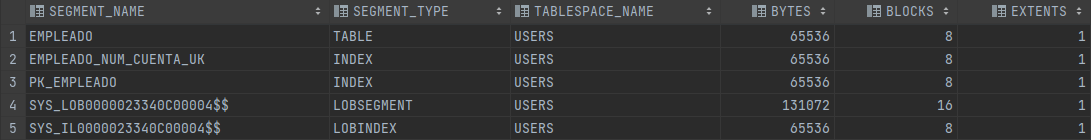
\includegraphics[scale=.22]{captura_2.png}
   \caption{T02\_DISPATCHER\_CONFIG}
   \label{fig:validador_2}
\end{figure}
\begin{figure}[H]
  \centering
  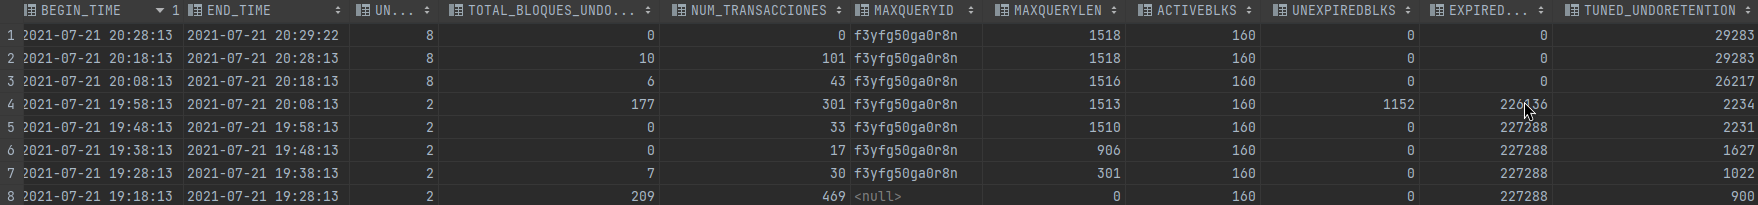
\includegraphics[scale=.18]{captura_3.png}
   \caption{T03\_DISPATCHER}
   \label{fig:validador_3}
\end{figure}
\begin{figure}[H]
  \centering
  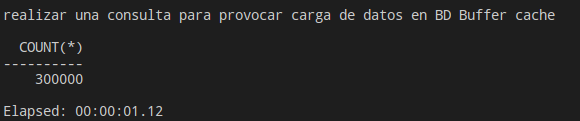
\includegraphics[scale=.18]{captura_4.png}
   \caption{T04\_SHARED\_SERVER}
   \label{fig:validador_4}
\end{figure}
\begin{figure}[H]
  \centering
  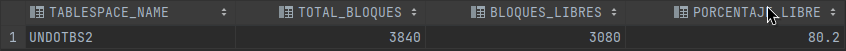
\includegraphics[scale=.18]{captura_5.png}
   \caption{T05\_QUEUE}
   \label{fig:validador_5}
\end{figure}
\begin{figure}[H]
  \centering
  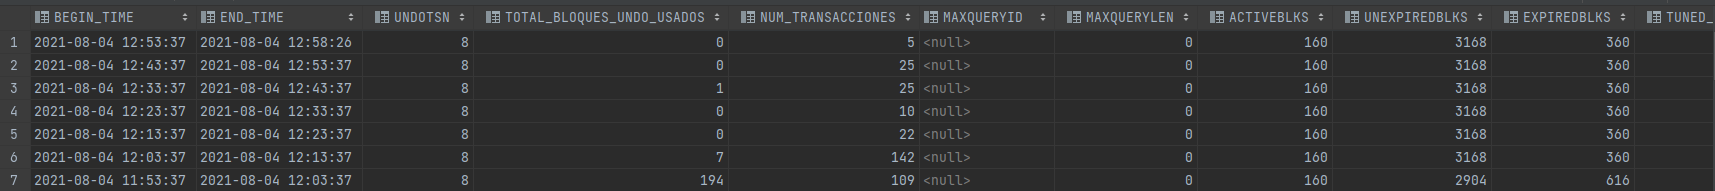
\includegraphics[scale=.18]{captura_6.png}
   \caption{T06\_VIRTUAL\_CIRCUIT}
   \label{fig:validador_6}
\end{figure}
\subsection{C4. Respuesta inciso A y s-04-procesos.sql}
\begin{lstlisting}[language=sql, caption=s-04-procesos.sql,label={lst:codigo6}]
whenever sqlerror exit rollback
set serveroutput on
connect sys/system2 as sysdba

declare
  v_count number;
  v_username varchar2(30) := 'VRA0501';
  v_table1 varchar2(30) := 'T07_SESSION_INFO_CONTEXT';
  v_table2 varchar2(30) := 'T08_SESSION_INFO_VIEW';
  v_table3 varchar2(30) := 'T09_PROCESS_INFO';
  v_table4 varchar2(30) := 'T10_BACKGROUND_PROCESS';
  v_table5 varchar2(30) := 'T11_FOREGROUND_PROCESS';
begin
  --Verificar si la table existe
  select count(*) into v_count
  from all_tables
  where table_name = v_table1
  and owner = v_username;
  --Si existe la tabla, entonces se borra
  if v_count > 0 then
    execute immediate 'drop table '|| v_username ||'.'||v_table1;
  end if;

  --Verificar si la table existe
  select count(*) into v_count
  from all_tables
  where table_name = v_table2
  and owner = v_username;
  --Si existe la tabla, entonces se borra
  if v_count > 0 then
    execute immediate 'drop table '|| v_username ||'.'||v_table2;
  end if;

  --Verificar si la table existe
  select count(*) into v_count
  from all_tables
  where table_name = v_table3
  and owner = v_username;
  --Si existe la tabla, entonces se borra
  if v_count > 0 then
    execute immediate 'drop table '|| v_username ||'.'||v_table3;
  end if;

  --Verificar si la table existe
  select count(*) into v_count
  from all_tables
  where table_name = v_table4
  and owner = v_username;
  --Si existe la tabla, entonces se borra
  if v_count > 0 then
    execute immediate 'drop table '|| v_username ||'.'||v_table4;
  end if;

  --Verificar si la table existe
  select count(*) into v_count
  from all_tables
  where table_name = v_table5
  and owner = v_username;
  --Si existe la tabla, entonces se borra
  if v_count > 0 then
    execute immediate 'drop table '|| v_username ||'.'||v_table5;
  end if;
end;
/
create table vra0501.t07_session_info_context(
    host varchar2(20),
    os_user varchar2(30),
    user_id number,
    session_id number
);

insert into vra0501.t07_session_info_context(host, os_user, user_id,session_id)
    select sys_context('USERENV','HOST') as host,
    sys_context('USERENV','OS_USER') as os_user,
    sys_context('USERENV', 'SESSION_USERID') as user_id,
    sys_context('USERENV','SID') as session_id
    from dual;

create table vra0501.t08_session_info_view as(
  select s.sid as session_id,s.paddr as process_address,
  s.username bd_username,s.status as session_status,
  s.port as client_port,s.process as os_client_process_id, 
  s.program as client_program from v$process p 
  join gv$session s on p.addr=s.paddr 
  join (select sys_context('USERENV','SID') as session_id
  from dual) c on c.session_id=s.sid where s.username = 'SYS'
);

create table vra0501.t09_process_info as(
    select sosid,pname,background, tracefile from v$process
	join gv$session s on addr=s.paddr join ( 
    select sys_context('USERENV','SID') as session_id
    from dual) c on s.sid = c.session_id 
);

create table vra0501.t10_background_process as(
    select addr, sosid, pname,username as os_username, background 
    from v$process where background='1'
);

create table vra0501.t11_foreground_process as(
    select p.addr, p.sosid, p.pname, p.username as bd_username, s.osuser as os_username, p.background 
    from v$process p left outer join v$session s 
    on(p.addr=s.paddr) where p.background is null
);

whenever sqlerror continue
\end{lstlisting}
\begin{figure}[H]
  \centering
  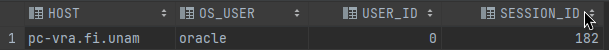
\includegraphics[scale=.25]{captura_7.png}
   \caption{T07\_SESSION\_INFO\_CONTEXT}
   \label{fig:validador_7}
\end{figure}
\begin{figure}[H]
  \centering
  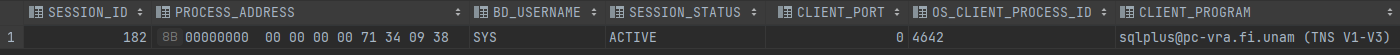
\includegraphics[scale=.17]{captura_8.png}
   \caption{T08\_SESSION\_INFO\_VIEW}
   \label{fig:validador_8}
\end{figure}
\begin{figure}[H]
  \centering
  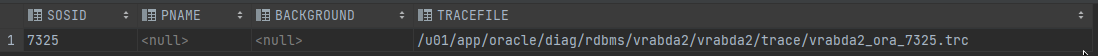
\includegraphics[scale=.20]{captura_9.png}
   \caption{T09\_PROCESS\_INFO}
   \label{fig:validador_9}
\end{figure}
\begin{figure}[H]
  \centering
  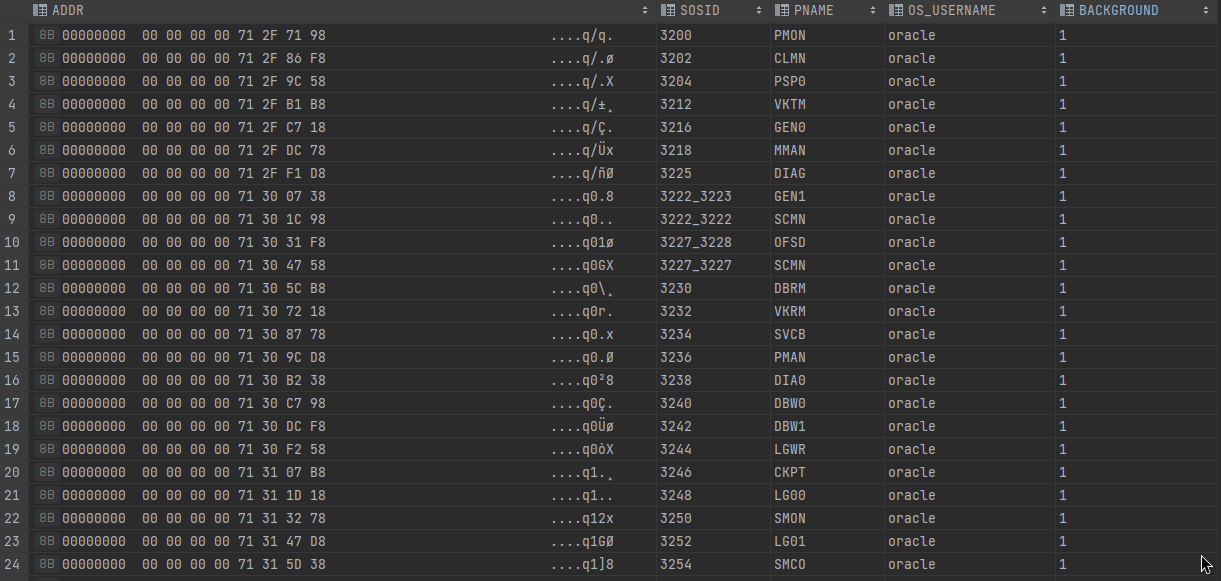
\includegraphics[scale=.20]{captura_10.png}
   \caption{T10\_BACKGROUND\_PROCESS}
   \label{fig:validador_10}
\end{figure}
\begin{figure}[H]
  \centering
  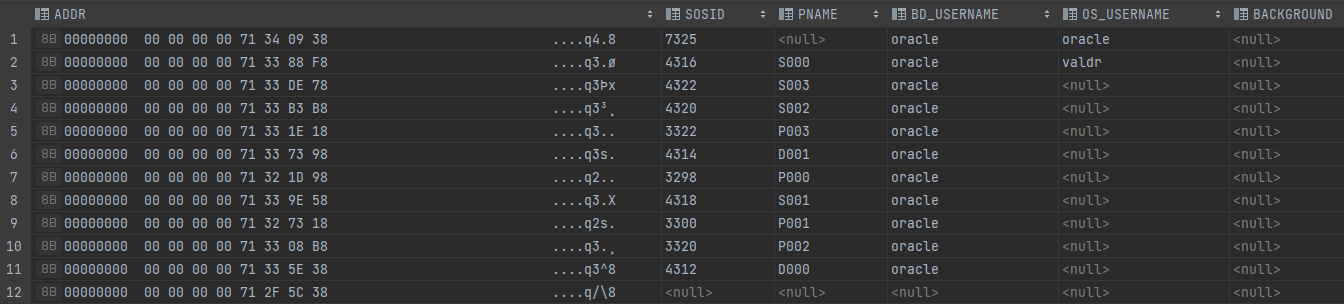
\includegraphics[scale=.18]{captura_11.png}
   \caption{T11\_FOREGROUND\_PROCESS}
   \label{fig:validador_11}
\end{figure}
\begin{lstlisting}[language=bash, caption=instrucciones SO,label={lst:codigo7}]
ps -ef | grep oracle
\end{lstlisting}
\section{Conclusiones}
\ifCLASSOPTIONcaptionsoff
  \newpage

\fi

\end{document}
